% Simposium MATHEMATICS and APPLICATIONS
% Requires Latex2e!
\documentclass[eng]{simposium}
\volume{,Vol. X}  %%%%%% TO BE ENTERED BY THE EDITOR(S)
\issue{(1)}      %%%%%% TO BE ENTERED BY THE EDITOR(S)
\pubyear{2019}   %%%%%% TO BE ENTERED BY THE EDITOR(S)
\firstpage{1}    %%%%%% TO BE ENTERED BY THE EDITOR(S)
\lastpage{12}     %%%%%% TO BE ENTERED BY THE EDITOR(S)

%%%%%% ENTER HERE ADDITIONAL PACKAGES
%%%%%% For example: \usepackage{gclc}

%%%%%% ENTER HERE YOUR OWN LATEX COMMANDS
%%%%%% For example: \newcommand{\const}{\mathop{\mathrm{const}}}

\begin{document}
\begin{frontmatter}

\title{Modified hybrid genetic algorithm for training convolutional neural networks}

\author{\textbf{\fnms{Milan M.} \snm{Čugurović}}}
\address{Faculty of Mathematics, University of Belgrade, Studentski trg 16, 11000 Belgrade\\
\email{milan\_cugurovic@matf.bg.ac.rs}
}
\author{\textbf{\fnms{Nikola} \snm{Dimitrijević}}}
\address{Microsoft Development Center Serbia, Španskih boraca 3, 11000 Belgrade\\
\email{nikoladim95@gmail.com}
}
\author{\textbf{\fnms{Stefan} \snm{Mišković}}}
\address{Faculty of Mathematics, University of Belgrade, Studentski trg 16, 11000 Belgrade\\
\email{stefan@matf.bg.ac.rs}
}

\received{\smonth{December} \syear{2019}}   %%%%%% TO BE ENTERED BY THE EDITOR(S)

\maketitle
\begin{abstract}
    
This paper presents a modified variant of genetic algorithm for training convolutional architectures which reduces the execution time of the algorithm. 
Modification is based on changing the evolutional segment of the algorithm by focusing on limiting the training time of each individual and incorporating the 
learnt knowledge of neuron parameters from the previous generations into each new one. By doing so the evolution is made more efficient, thus reducing the time 
needed to find the desired architecture.

Additional contribution of this paper is creating new dataset \textit{DoubledMNIST}, which represents a successor of the popular MNIST dataset.
Created dataset is doubled with respect to the MNIST dataset both in terms of the number of instances and in terms of the resolution of each individual isntance.
Results shown in the paper were obtained using the presented improved method on the created dataset. The paper also shows classification results on the said dataset.
\end{abstract}

\begin{keyword}
genetic algorithm; CNN arhitectures; MNIST dataset; DoubledMNIST dataset
\end{keyword}
\end{frontmatter}

\section{Introduction}

Inspirisani modernim trendovima u razvoju dubokih konolutivnih neuronskih arhitektura \cite{28}\cite{29} istrazivaci u 
oblasti masinkog ucenja vec dugo pokusavaju naci sisteme koji ce automatski generisati pogodne arhitekture dubokih 
neuronskih mreza, koje bi sa jedne strane imale dovoljne kapacitete (u smislu mogucnosti ucenja odnosno broja parametara) dok 
bi sa druge strane bile lake za obucavanje i propagaciju gradijenata. Jedan nacin prustupa resavanju ovog problema jesu genetski 
algoritmi odnosno simulacija evolucije kojom bi se favorizovale arhitekture koje su u stanju da se brzo prilagode, adaptiraju 
i ispune prethodne uslove. Ovaj pristup dao je jako dobre rezultate \cite{5}\cite{30}\cite{31}. Za neke usko specificne oblasti 
jako dobri rezultati dobijeni su kombinovanjem ova dva pristupa \cite{32}\cite{33} sto je pokazalo da su one jako kompatibilne. 

Sa druge strane, evolutivni algoritmi, koji se u sustini zasnivaju na simulaciji prirodne evolucije, te stoga zatevaju jako 
veliki broj generacija i dodatno veliki broj jedinki u svakoj od njih komplementarni su sa arhitekturama dubokog ucenja, konkretno 
sa dubokim konvolutivnim neuronskim mrezama, s obzirom da one obicno imaju jako puno parametara, zbog cega zahtevaju veliku 
kolicinu vremena da bi se optimizovale. Stoga je najveca prepreka prilikom integracije ova dva pristupa upravo vreme potrebno 
za obucavanje svake jedinke genetskog algoritma. U ovom radu pokazali smo da je zaista moguce resiti ovaj problem ukoliko se 
jedinkama jedne generacije dopusti preuzimanje znanja njihovih roditelja. Ovime smo osvarili ubrzanja do reda velicine dva. pri 
nekim scenarijima evolucije. Dodatno, pokazali smo da je moguce iskoristiti naucene arhitektute koje su se dobro pokazale na jednom 
za treniranje i na novim, slicnim skupovima poidataka.

U to ime kreirali smo i novi skup podataka, za koji smatramo da ce postati naslednik sada vec viralnog skupa podataka MINST.

U poglavlju 2 dat je osvrt na prethodni rad u oblasti, poglavlje 3 do detalja opisuje skup pdoataka koji smo kreirali, 
u poglavlju 4 diskutuje se predlozeni metod poboljsanja, dok su u poglavlju 6 dati konkretni rezultati dobijeni evaluacijom 
predlozenog pristupa. Poglavlje 6 predstavlja zakljucak, rekapitulira uradjeno i dalje smernice za dalja poboljsanja. 

\textcolor{red}{da spomenemo izvor ideje?}

\textcolor{blue}{Mislis rad genetic cnn?}

\section{Related work}

This section provides background about offline handwritten character datasets and about incorporating genetic algorithms 
with the learning of CNN architectures, and their training. 

\subsection{Offline Handwritting Datasets}

The existence of quality datasets of handwritten characters is a prerequisite for the development of quality handwriting 
recognition techniques and their evaluations in different research scenarios. 
The task of collecting this kind of data is very demanding and arduous, since in order to create a dataset that includes 
a variety of writing styles, a large number of respondents must be involved. 
The process of creating handwritten databases began in the 1990s\cite{9} and is still ongoing. 
In the meantime, a large number of datasets have been developed. 

Some of the most important and commonly used datasets of offline handwritten characters are: CVL database \cite{18}, RIMES database \cite{10}, IAM dataset \cite{11}, 
NIST \cite{12}\cite{13}, MNIST \cite{8} and EMNIST \cite{1} datasets, CEDAR \cite{14}, UNIPEN \cite{15}, IBM UB \cite{16} and so on. 
Although the most commonly used datasets are datasets of handwritten Latin/English alphabet 
there are significant datasets from other alphabets. 
Here we refer to datasets of handwritten Chinese \cite{19}\cite{20}\cite{21}, Arabic \cite{22}\cite{23}, as well as Bangala \cite{24}\cite{25} datasets, while there are many others. 
In addition, the development of multilingual datasets has been intensively developing in the last few years \cite{17}\cite{26}\cite{18}, which seeks to create an alphabet independent handwriting recognition system. 
A more detailed overview of handwritten character datasets can be found in \cite{9}, 
while the datasets of the NIST family will be described in more detail below, since the dataset we created was built on the same basis. 

\subsubsection{NIST dataset}

NIST Special Database 19 \cite{12}\cite{13} was developed by the American National Institute of Standards and Technology as CD-ROM in 1995, and then was 
re-released in 2016 using modern file formats. 
This offline database of handwritten digits and numerals contains $815255$ segmented characters, each labeled 
with one of $62$ classes ($10$ digits, $26$ lowercase and $26$ uppercase English alphabet characters). 
Those segmented characters are represented as monochromatic images, in resolution $128$ by $128$ pixels. 
Each of individual images were obtained from one of the $3669$ completed forms (an example of one such is given in the figure \ref{fig:nist}), 
where the segmentation of each of the images was checked manually. 
The database contains characters from $3596$ authors. 
The database is provided through several hierarchies and it is suitable for the tasks of author identification, handwriting recognition, etc. 
The authors also proposes internal division of data for training and testing 
(recommended data for testing comes from high school students' handwriting). 

\begin{figure}[!ht]
  \centering
  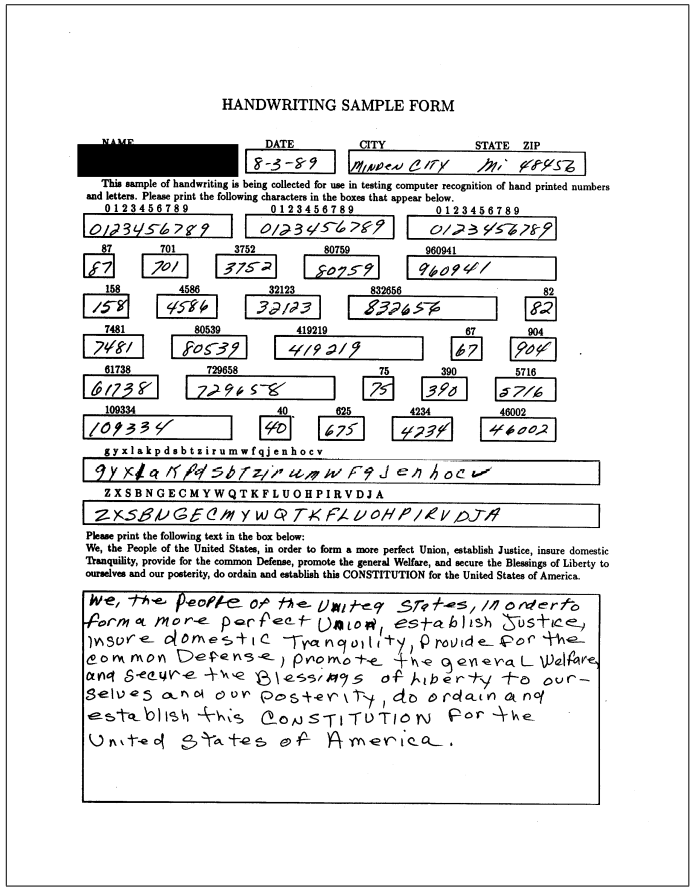
\includegraphics[width=0.65\textwidth]{nist.png}
  \caption{One of the NIST data gathering forms \cite{9}}
  \label{fig:nist}
\end{figure}

\subsubsection{MNIST dataset}

The MNIST dataset of offline handwritten digits, developed by Le Cun et all. in 1998 \cite{8}, has become on of the most famous and the most important dataset in machine learning, 
classification and computer vision tasks. 
MNIST was the first famous dataset derived from the larger NIST Special Database 19. 
The dataset contains $60,000$ images in the training set and $10,000$ images in the test set, labeled with one out of ten possible digits. 
The images are in grayscale, measuring $28$ times $28$ pixels. 
The images of the MNIST training and test set were created uniformly from the NIST training and test set, 
by selecting $50\%$ of the images from each, while maintaining the identical distribution of the MNIST training and test part. 
Over the years, this dataset has been widely used both in a large number of digit recognition systems and as a core dataset 
when introducing basic machine learning and pattern recognition concepts. 

\subsubsection{EMNIST dataset}

The Extended MNIST (EMNIST) dataset represents a younger dataset created from the NIST database. 
It was created in 2017 by Cohen et al. \cite{1}. 
It consists of several sub-datasets: EMNIST By\_Class and EMNIST By\_Merge Datasets, EMNIST Balanced Dataset, 
EMNIST Letters Dataset and EMNIST MNIST Dataset. 
The images in each of them are monochromatic and are in resolution $28$ times $28$ pixels, 
while depending on the dataset, the labels to which they are marked differ. 
The EMNIST By\_Class and By\_Merge datasets both contains all NIST images, but differ in number of labels and images distribution 
in each of the label. By\_Class dataset contain images labeled with $62$ classes (NIST like), while in By\_Merge dataset 
the upper and lower case examples for the classes C I J K L M O P S U V W X Y Z have been merged. 
EMNIST Balanced dataset contains of $131,600$ images labeled with one of the $47$ classes. 
This dataset is created intend to avoid misclassification errors caused by lower-upper versions of the same character. 
EMNIST Letters dataset consists of images labeled with one of the $26$ English alphabet classes 
(uppercase and lowecase letters are merged like some classes in prevous sub-dataset). 
EMNIST MNIST dataset contains of $280,000$ MINST like images, labeled with $10$ digits classes. 

The same conversion process was used when creating each of the sub-datasets. 
The authors simulated the conversion process that was used in creating the MNIST dataset, in order 
to share the same structure. 
The process of converting NIST images involves sequentially adding Gaussian noise (which the standard deviation parameter set to 1), 
extracting regions around a character, character centering, resizing, and resampling to obtain an image with the appropriate MINST-like dimensions. 

The impact of the MNIST dataset is also evident in the fact that there are datasets in other areas (such as computer vision) that
follows the same structure and are named like this viral dataset \cite{27}. 
In this paper we introduce MINST like dataset, but doubled in number of samples and in resolution each of them. 
The created dataset, which we called \textit{Doubled MNIST}, is fully described in Section 3. 

\subsection{Genetic CNN}

With the rise in number of layers in the CNNs, deeper neural networks are more difficult to train, and using skip connections proved invaluable and allowed 
for easier training of substantially deeper networks \cite{6}. Those skip connections enable identity functions to be learned easily where needed.
Those skip connections can be manually selected, but since the number of possible skip connections grows exponentially, and because evaluating each model can take a long time, 
in practice its impossible to try each possible architecture.
Many handcrafted CNN architectures exist, but since manually searching the space of all architectures is impractical, it gives a great incentive for automatic search 
for a good architecture.

A possible solution for finding a good architecutre automatically is by using some kind of metaheuristic. 
One paper proposes an encoding method of representing each network structure as a fixed length binary string \cite{4}. 
They define genetic operations: selection, mutation and crossover to generate better suited individuals and eliminate weak ones.
The fitness of an individual is defined through as their recognition accuracy, which is gathered through evaluation on a given reference dataset.
The learnt structures are transferrable to other datasets image-baseed datasets.

Another approach focuses on automatically constructing CNN architectures for an image classification task based based on Cartesian genetic programming (CGP).
They use convolutional blocks and tensor concatenation as the node functions in CGP. Their results are comparable with handcrafted state-of-the-art models \cite{5}.

\section{\textit{DoubledMNIST Dataset}}

After developing an architecture that solves the classification task on MNIST dataset, the natural next step of learning is 
to modify it to solve classification tasks on similar datasets. 
This was one of the basic motives that inspired us to create this kind of dataset. 
In addition, we aimed to create a dataset that is simple in structure (like a MNIST dataset) but still of more demanding 
dimensions, which would highlight all the advantages and disadvantages of various classification techniques that can be 
applied to it, which on the other hand would be really nice a dataset for an introduction to machine learning. 
On the other hand, the dimensions of the created data set as well as its structure and complexity qualify it for more 
serious applications than just educational ones. 
One of the reasons why the MNIST dataset has become very popular was its dimensions, which are extremely suitable for 
testing different types of deep learning architectures \cite{27}. 
Our idea was that create dataset that would serve as the second phase of testing in the development of those architectures, 
which, after the MNIST, would have to satisfy the more difficult requirements of our data set. 

The created dataset consists of $140,000$ images, $120,000$ in the training set and $20,000$ in the test set. 
All images are monochromatic, measuring $56$ times $56$ pixels. 
Each image, as in the MNIST dataset, is labeled with one out of ten labels (digits from $0$ to $9$). 
A random sample of our database images is given in the figure \ref{fig:nist_sample}. 

\begin{figure}[!ht]
  \centering
  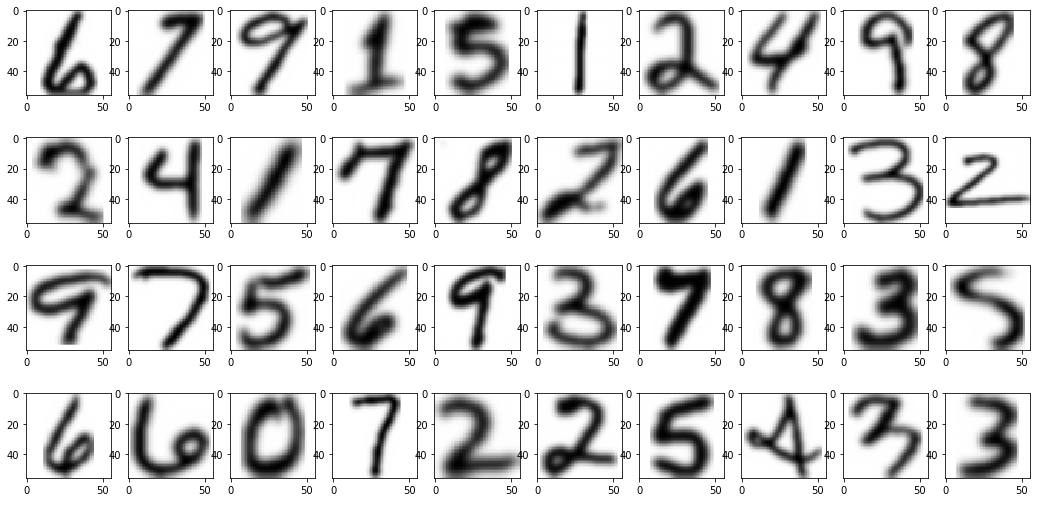
\includegraphics[width=1\textwidth]{sample_from_nist.png}
  \caption{Sample of images from the DoubledMNIST database.}
  \label{fig:nist_sample}
\end{figure}

Each image in our dataset was created by processing images of the NIST database, 
mostly following the instructions given in \cite{1}, which in turn follow the same conversion process described in \cite{8}. 
For each of the ten digits, our conversion process first randomly selects $14,000$ images corresponding to it from the NIST 
database ($12,000$ for a Doubled MNIST training set and $2,000$ for a Doubled MNIST test set), which we later transform 
from pixel binary images in resolution $128$ times $128$ to an 8-bit gray-scale images in resolution $56$ times $56$. 
We used a random selection of which of the photographs from the NIST database would be in our dataset just to avoid possible 
bias to individual writers' groups and their handwriting. 

After loading the chosen image from the NIST dataset, the character itself is first cropped using a two pixel padding. 
We have taken the actual value of the offset from the publication we already mentioned, and their conversion process \cite{1}. 
Thereafter, to soften the character borders, we blured cropped image using a Gaussian filter with standard deviation set to $2$. 
A border frame is then placed around a character that is so extracted. 
It is important to emphasize here that the dimensions of the border frames differ greatly, since the dimension of the 
character is certainly one of the characteristics of the manuscript. 
Following the principles used in \cite{1} we tried to use the maximum amount of space available, and 
therefore we did not downsample the cropped characters into smaller resolutions before the final one. 
Instead we then convert the cropped image of dimensions \textit{height} $\times$ \textit{width} into a square image of dimensions 
\textit{max(height, width)} $\times$ \textit{max(height, width)} by extending the shorter dimension with the blank pixels 
while keeping the character centered in the image. 
The next step was to resize an image of dimensions \textit{max(height, width)} $\times$ \textit{max(height, width)} into a 
dimensions $56 \times 56$.
We did this downsampling using bi-cubic interpolation. 
Finally, the image pixels are scaled into the 8-bit range. 
An example of the conversion described above is given in Figure \ref{fig:conversion}. 

\begin{figure}[!ht]
  \centering
  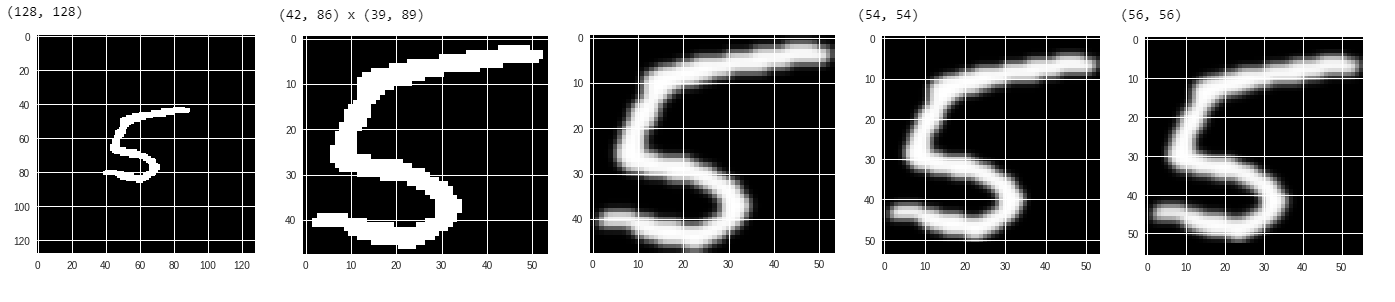
\includegraphics[width=1\textwidth]{conversion.png}
  \caption{Conversion process: 
  (1) original $128 \times 128$ NIST binary images; 
  (2) cropped character with padding set to $2$; above the image we can see pixel indices that represent the boundaries of our character in the original image; 
  (3) character after applying Gaussian filter with sigma set to $2$; 
  (4) image centered into a squared \textit{max(height, width)} $\times$ \textit{max(height, width)} frame; 
  (5) image sampled in resolution $56 \times 56$ using bi-cubic interpolation}
  \label{fig:conversion}
\end{figure}

Additionally, while creating this dataset, we tried various combinations of noise addition and interpolation. 
Some of the variations we applied were: used Gaussian noise and Bicubuc interpolation, Gaussian noise with Lanczos interpolation 
and Bilinear interpolation, Bicubic interpolation with Gaussian Laplace filter and Fourier Gaussian filter and so on. 
We evaluated the quality of each combination by training a simple model of K Nearest Neighbors in the images modified by that 
combination. We chose the first variant, just like in the paper \cite{1}, but we used the standard deviation set to $2$ 
instead of $1$ as much as they used in the mentioned paper (since such a filter achieved better results through our evaluations). 

\section{Network representation}
\label{sec:repr}

Many network architectures, such as \cite{6,7}, can be partitioned into stages.
In each stage the width, height and depth of the data cube remain unchanged. 
Adjacent stages are connected with pooling layers which reduce both width and height of the data.
The polling usually performs $2 \times 2$ max polling operation, which halfs the width and height by transforming each $2 \times 2$ 
pixel group into one pixel whose value is the maximum of the pixel group.
The number of channels (filters) within convolutions of the same stage is the same.

That observation is leveraged to define a set of networks which 
can be encoded into a binary string of fixed length. 
Couse of that, in our work we used the binary string network representation which was proposed in \cite{4}. 
In our scenario, a CNN is composed of $S$ stages, each containing 
$K_i$ nodes ($i=1,...,S$). 
The nodes within a stage are ordered, and connections are only allowed from a lower number towards a higher numbered node.
Each node represents a convolutional operation. If a node has multiple inputs, then they are all summed up element-wise.
After convolution the ReLU activation is performed. 
The fully connected end of the network is not encoded, as its hyperparameters are static. 

Since each node can be an input only to higher nubmered nodes, that means that 
$(K_i -1) + (K_i - 2) + ... + 2 + 1 = \frac{K_i(K_i-1)}{2}$ bits are needed to encode a stage containing $K_i$ nodes.

Some encodings would represent invalid networks, thus default nodes are introduced in each stage.
They are the first and the last nodes in the stage, and since they're always present, they aren't encoded in the binary string.

There are a few special cases:
\begin{itemize}
    \item If a node does not have any input or output, then it is removed.
    \item If a node does not have an input, then we connect the first node in the stage to it.
    \item If a node does not have an output, then we connect it to the last node in the stage.
\end{itemize}

We have adapted our genetic algorithm so that the chromosome is represented by a binary string representing 
the architecture of the convolutional part of the neural network, which we defined as described above. 

\section{Method}

The core idea of the genetic algorithm is to get a good solution to a problem by generating increasingly better solutions through the process of evolution.
Network architecture is encoded as a binary string of fixed length. That string represents a gene of an individual.
Individuals from the population have a higher chance to pass on their genes to the next generation if they are more fit for a given task.
Through many generations its expected to arrive to a population that has many good individuals and the best individual out of that last generation represents the solution.

The evolution process consists of selection, mutation and crossover. 
The selection process allows stronger individuals to be perserved, and for weaker individuals to be eliminated.
Crossover process combines genes of two individuals to create individuals for the new generation.
Mutation randomly changes a gene of an individual, thus introducing more variety within a population.


\begin{algorithm}[H]
  \SetAlgoLined
  \textbf{Input:} the testing dataset $T$, number of generations $G$, number of individuals in each generation $N$,
  mutation and crossover probabilities $p_M$ and $p_C$, mutation parameter $q_M$ and crossover parameter $q_C$.

  \textbf{Initialization:} generate randomized individuals, train them and compute their fitness (evaluate classification accuracy)\;
      \For{t = 1,...,$G$}{
          \textbf{Selection:} perform selection using a rulet method to p\;
          \textbf{Crossover:} perform crossover with probability $p_C$ and crossover parameter $q_c$\;
          \textbf{Mutation:} perform mutation on individuals which have not had crossover with probability $p_M$ and mutation parameter $q_M$\;

          \textbf{Construction:} construct CNN from the gene encoding it\;
          \textbf{Inheritance:} inherit the stage weights from the most similar individual of the last generation\;
          \textbf{Training:} train the constructed networks, where number of epochs depends on number of inherited stages\;
          \textbf{Evaluation:} evaluate all individuals to get their fitness\;
   }
   \textbf{Output:} individuals of the final generation and their classification accuracy.
   \caption{Genetic algorithm for generating the appropriate network architecture}
\end{algorithm}


We denote the $n$-th individual in generation $t$ as $M_{t,n}$ and fitness of that individual as $f_{t,i}$.

\subsection{Initialization phase}
The initial generation of individuals is generated by assigning each bit in the binary string a random value from Bernoulli distribution $\mathcal{B}(0.5)$.
Then all individuals from the initial generation are fully trained on the training dataset and evaluated on a testing dataset to get their fitness.
After that, the genetic evolution process is repeated for a set number of generations.

\subsection{Selection phase}
The most common selection methods are roulet selection and tournament selection. 
Here we use roulet selection where the least fit individual is always eliminated.
In roulet selection, each individual has a chance to pass on its genes to the next generation, 
where the probability of that event is proportional to the individuals fitness in comparison to the fitness of all other individuals.
The sampling is performed $N$ times (number of individuals in each generation) with replacement, thus each individual may be selected multiple times.
The probability of individual $M_{t,n}$ passing the selection is equal to $f_{t,i} / \sum_{i=1}^{N} (f_{t,i} - f_{t,min}$), where $f_{t, min} = \min_{i=1}^{N} {f_{t,i}}$.

\subsection{Crossover phase}
The crossover process combines the genes of two individuals to create one or two new individuals.
Here crossover of two individuals always results in two new individuals.
When two individuals are in a crossover they swap a whole stage.
That way the learned connections within a stage are kept through the generations, while still introducing more variaty in individuals.
Candidates for crossover are pairs of individuals $(M_{t,2i-1}, M_{t,2i}), \forall i=1,..,\lfloor N/2\rfloor $.
The probability of crossover between two individuals is $p_C$, and the probability of two stages being swapped is $q_C$.

\subsection{Mutation phase}
Mutation can occur only if an individual didn't go through the crossover process.
In that case the individual starts going through mutation with probability $p_M$.
Then each bit in the individuals string representation has a low chance of being inverted, defined in $q_M$.
Mutation ensures additional variaty in individuals and allows for exploring different architectures within each stage.

\subsection{Construction phase}
The binary encoded  string of each individual is parsed and the graph is constructed, where graph nodes represent the convolution operations.
Connections withing graph nodes signal that there is a connection between those two nodes.
The whole CNN is constructed by parsing the binary string according to the representation discussed in \ref{sec:repr}. 
The end of the network always consists of a flatten layer, followed by a dense (fully connected) layer with 32 units, and finally a dense 
layer with softmax activation and number of units equal to the number of possible classes.

\subsection{Training phase}
Training is performed on a constructed CNN model for a set amount of epochs. 
The more stages were inherited in inheritance phase, the less number of epochs is needed to train the model.
Training is done on the training dataset which is the same for all individuals.

\subsection{Evaluation phase}
Evaluation phase is performed to get the fitness of an individual.
The trained model is evaluated on a testing dataset to get its classification accuracy, which is used as its fitness.

%todo moraju od pocetka segmenti opisi`
\section{Evaluation}

In this section we will describe the results we achieved using proposed method. 
We evaluated our model on the MNIST dataset \cite{8}. In addition, we trained the learned architecture on the 
created dataset DoubledMNIST, thus defining the first classification results on it. 
Additionally, all of our source code is publicly available at the web address \textit{github.com/MilanCugur/Genetic\_Evolution\_For\_CNN}. 

The choice of architecture was made on the mnist dataset, given its characteristics. 
When choosing the architecture, three convolutional stages with $3$, $4$ and $5$ convolutions respectively were used. 
Previously indicates that architectures are represented by the genome with a length of $19$.
The number of filters is the same for each convolution in the same stage, and is equal to $32$ $48$ and $64$, respectively, across the stages. 

When evaluating the proposed method, we created several different benchmarks that cover several basics evolution scenarios. 
In each of them, the proposed method gave a significant improvement. 
Specific scenarios and results are given with:
\begin{itemize}
  \item 4 individuals trained over 4 generations: baseline training time: $32$min $44$sec, proposed method training time: $18$min $01$ sec
  \item 20 individuals trained over 20 generations: baseline training time: $2$h $33$min $54$sec, proposed method training time: $1$h $06$min $25$ sec
  \item 2 individuals trained over 20 generations: baseline training time: $25$min $25$sec, proposed method training time: $18$min $18$ sec
  \item 20 individuals trained over 2 generations: baseline training time: $1$h $22$min $22$sec, proposed method training time: $46$min $55$ sec
\end{itemize}

In the previous list, the first two points correspond to the scenario when we have an identical 
(in the first point insufficient but in the second point sufficient) number of generations and individuals in them. 
In the second point, only one sixth of the MNIST dataset was used because of the computational complexity and limitations of our machine. 
The third point simulates an evolution scenario when we have enough individuals, however a very short number of generations, 
while the last point simulates the opposite situation when the number of generations is sufficient, but when we do not have 
enough individuals in them. 
It is important to point out that in each of the four preceding scenarios, our re-presented method has yielded a significant 
improvement measured in time savings, without losing out on the quality of the generated architectures. 

The standard evolution scenario when we have enough ($10$) individuals in each of the $10$ generations of evolution 
(trained across the entire MNIST dataset) generated the architectures as in Figure \ref{fig:architectures}, 
while the results of the two best individuals of each generation can be seen in Figure \ref{fig:top2}. 

\begin{figure}[!ht]
  \centering
  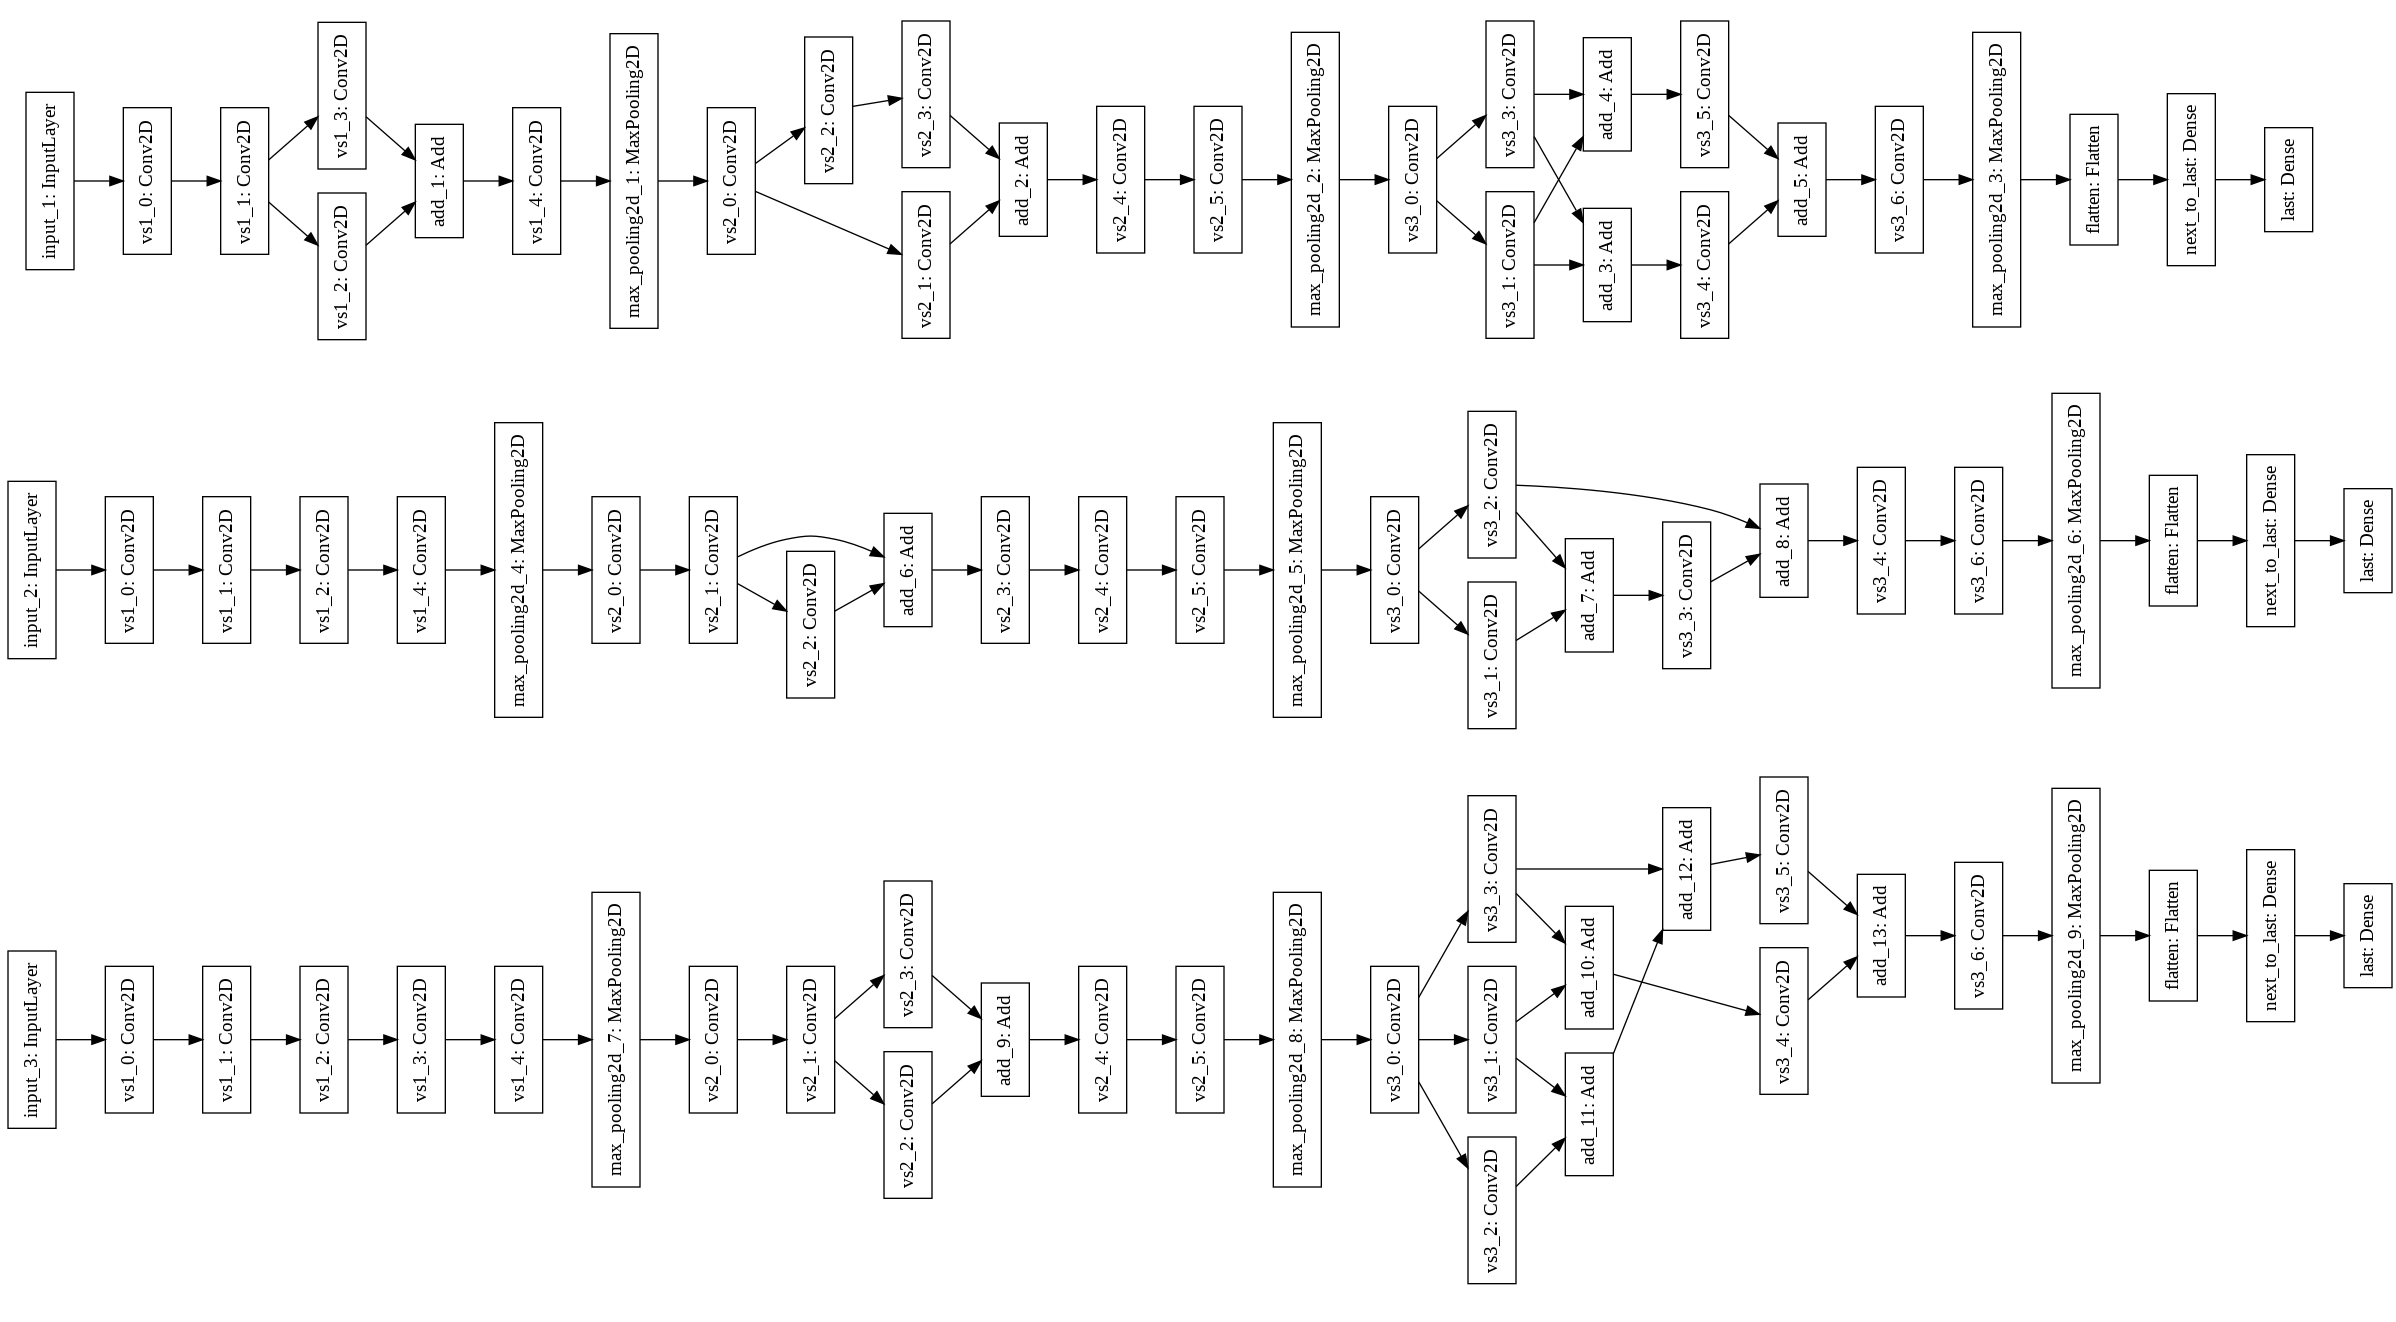
\includegraphics[width=1\textwidth]{arhitekture.png}
  \caption{Generated architectures using presented method on NIST dataset}
  \label{fig:architectures}
\end{figure}

\begin{figure}[!ht]
  \centering
  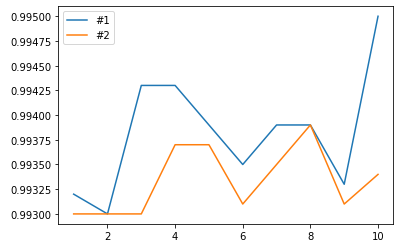
\includegraphics[]{top1.png}
  \caption{Top two individuals precision through ten GA trining epochs}
  \label{fig:top2}
\end{figure}

The first architecture of Figure \ref{fig:architectures} was trained on a DoubledMNIST dataset with training lasting about 
$30$min and stopped with an early stop technique after $14$ epochs, with $99.495\%$ precision on the test set. 
This sets the results of the cassification on the created dataset. 

\section{Conclusion}

U ovom radu pokazali smo da je moguce ubrzanje genetskog algoritma za treniranje dubokih konvolutivnih neuronskih mreza 
ukoliko jedinke jedne generacije koriste znanje (odnosno parametre) koje su naucili njihovi roditelji. 
Ukljucivanjem ovakvih roditelj-dete veza omogucili smo veliko smanjenje vremena izvrsavanja samog algoritma s obzirom da 
najveci deo vremena izvrsavanja genetski algoritmi ovog tipa trose u treninranju samih jedinki svake od generacija. 
Dodatno, redukovani trening koji izvodimo u slucaju nasledjivanja odredjenog broja prvih slojeva mreze od jednog od roditelja 
doprinosi robusnosti samog procesa treninga jer se prvi slojevi finalne mreze koji definisu nove atribute nad kojima dublji 
slojevi u mrezi uce retreniraju kroz nekoliko epoha (koliko prezive). %% da li je prejaka poslednja tvrdnja?

Dodatno, testovi koje smo izveli pokazali su da se nas sistem ponasa izuzetno dobro pri raznim scenarijima evolucije, 
kada imamo dovoljno i vremena i jedinki, u situacijama kada nam je broj generacija iz nekog razloga ogranicen ali imamo dovoljno 
veliku populaciju, kao i u situaciji kada imamo dovoljno vremena za evoluciju ali je broj samih jediniki u populaciji ogranicen.

Jos jedan doprinos ovog rada jeste kreiranje novog skupa oflajn rukom pisanih karaktera engleskog alfabeta koji treba da bude 
naslednik popularnog skupa podataka MINST, s obzirom na svoje dimenzije i karakteristike. Kreirani skup podataka idealan je 
za zadatke ucenja masinskog ucenja, kada se arhitekture kreirane na MNISTU prilagodjavaju ozbiljnijim zahtevima koje pred 
algoritme stavlja nas skup podataka. 
Rezultati koje smo ostvarili trenirajuci arhitekturu dobijenu izvrsavanjem genetskog algoritma na skupu podataka MINST predstavljaju 
prve takve na skupu podataka DoubledMNIST.

\newpage

\begin{thebibliography}{99}
\bibitem{1}   
\textbf{Cohen, G., Afshar, S., Tapson, J., van Schaik, A.} EMNIST: an extension of MNIST to handwritten letters. \emph{arXiv preprint arXiv:1702.05373.}, 2017.

\bibitem{2} 
\textbf{Floreano, D., Dürr, P., Mattiussi, C.} Neuroevolution: from architectures to learning. \emph{Evolutionary intelligence}, 1(1), 47-62, 2008.

\bibitem{3} 
\textbf{Voß, S., Martello, S., Osman, I. H., Roucairol, C. (Eds.).} Meta-heuristics: Advances and trends in local search paradigms for optimization. \emph{Springer Science and Business Media.}, 2012.

\bibitem{4}
\textbf{Xie, L., Yuille, A. } Genetic cnn. \emph{In Proceedings of the IEEE International Conference on Computer Vision (pp. 1379-1388).}, 2017.

\bibitem{5}
\textbf{Suganuma, M., Shirakawa, S., Nagao T. } A genetic programming approach to designing convolutional neural network architectures. \emph{In Proceedings of the Genetic and Evolutionary Computation Conference (pp. 497-504).}, 2017.

\bibitem{6}
\textbf{He, K., Zhang, X., Ren S., Sun J.} Deep Residual Learning for Image Recognition. \emph{The IEEE Conference on Computer Vision and Pattern Recognition (CVPR)}, 2016.

\bibitem{7}
\textbf{Simonyan K., Zisserman A.} Very Deep Convolutional Networks for Large-Scale Image Recognition. \emph{International Conference on Learning Representations}, 2014.

\bibitem{8}
\textbf{LeCun Y., Bottou L., Benigo Y., Haffner P.} Gradient-based learning applied to document recognition., \emph{Proceedings of the IEEE, 86(11):2278-2324}, November 1998.

\bibitem{9}
\textbf{Hussain, R., Raza, A., Siddiqi, I., Khurshid, K., Djeddi, C.} A comprehensive survey of handwritten document benchmarks: structure, usage and evaluation. \emph{EURASIP Journal on Image and Video Processing, 2015(1), 46.}, 2015.

\bibitem{10}
\textbf{Grosicki, E., Carre, M., Brodin, J. M., Geoffrois, E.} RIMES evaluation campaign for handwritten mail processing., 2008.

\bibitem{11}
\textbf{Marti, U. V., Bunke, H.} The IAM-database: an English sentence database for offline handwriting recognition. \emph{International Journal on Document Analysis and Recognition, 5(1), 39-46.}, 2002.

\bibitem{12}
\textbf{Grother, P. J.} NIST special database 19. \emph{Handprinted forms and characters database, National Institute of Standards and Technology.}, 1995.

\bibitem{13}
\textbf{Grother, P. J.} NIST Special Database 19. \emph{NIST Handprinted Forms and Characters Database (No. World Wide Web-Internet and Web Information Systems).}, 2016.

\bibitem{14}
\textbf{Singh, S., Hewitt, M.} Cursive digit and character recognition in CEDAR database. \emph{In Proceedings 15th International Conference on Pattern Recognition. ICPR-2000 (Vol. 2, pp. 569-572). IEEE.}, 2000.

\bibitem{15}
\textbf{Guyon, I., Schomaker, L., Plamondon, R., Liberman, M., Janet, S.} UNIPEN project of on-line data exchange and recognizer benchmarks. \emph{In Proceedings of the 12th IAPR International Conference on Pattern Recognition, Vol. 3-Conference C: Signal Processing (Cat. No. 94CH3440-5) (Vol. 2, pp. 29-33). IEEE.}, 1994.

\bibitem{16}
\textbf{Shivram, A., Ramaiah, C., Setlur, S., Govindaraju, V.} IBM\_UB\_1: A dual mode unconstrained English handwriting dataset. \emph{In 2013 12th International Conference on Document Analysis and Recognition (pp. 13-17). IEEE.}, 2013.

\bibitem{17}
\textbf{Al Maadeed, S., Ayouby, W., Hassaïne, A., Aljaam, J. M.} Quwi: An arabic and english handwriting dataset for offline writer identification. \emph{In 2012 International Conference on Frontiers in Handwriting Recognition (pp. 746-751). IEEE.}, 2012.

\bibitem{18}
\textbf{Kleber, F., Fiel, S., Diem, M., Sablatnig, R.} Cvl-database: An off-line database for writer retrieval, writer identification and word spotting. \emph{In 2013 12th International Conference on Document Analysis and Recognition (pp. 560-564). IEEE.}, 2013.

\bibitem{19}
\textbf{Liu, C. L., Yin, F., Wang, D. H., Wang, Q. F.} CASIA online and offline Chinese handwriting databases. \emph{In 2011 International Conference on Document Analysis and Recognition (pp. 37-41). IEEE.}, 2011.

\bibitem{20}
\textbf{Su, T., Zhang, T., Guan, D.} HIT-MW dataset for offline Chinese handwritten text recognition., 2006.

\bibitem{21}
\textbf{Liu, C. L., Yin, F., Wang, D. H., Wang, Q. F.} Online and offline handwritten Chinese character recognition: benchmarking on new databases. \emph{Pattern Recognition, 46(1), 155-162.}, 2013.

\bibitem{22}
\textbf{Pechwitz, M., Maddouri, S. S., Märgner, V., Ellouze, N., Amiri, H.} IFN/ENIT-database of handwritten Arabic words. \emph{In Proc. of CIFED (Vol. 2, pp. 127-136). Citeseer.}, 2002.

\bibitem{23}
\textbf{Märgner, V., El Abed, H.}ICDAR 2009 Arabic handwriting recognition competition. \emph{In 2009 10th International Conference on Document Analysis and Recognition (pp. 1383-1387). IEEE.}, 2009.

\bibitem{24}
\textbf{Sarkar, R., Das, N., Basu, S., Kundu, M., Nasipuri, M., Basu, D. K.} CMATERdb1: a database of unconstrained handwritten Bangla and Bangla–English mixed script document image. \emph{International Journal on Document Analysis and Recognition (IJDAR), 15(1), 71-83.}, 2012.

\bibitem{25}
\textbf{Chaudhuri, B. B.} A complete handwritten numeral database of Bangla–a major Indic script., 2006.

\bibitem{26}
\textbf{Djeddi, C., Gattal, A., Souici-Meslati, L., Siddiqi, I., Chibani, Y., El Abed, H.} LAMIS-MSHD: a multi-script offline handwriting database. \emph{In 2014 14th International Conference on Frontiers in Handwriting Recognition (pp. 93-97). IEEE.}, 2014.

\bibitem{27}
\textbf{Xiao, H., Rasul, K., Vollgraf, R.} Fashion-mnist: a novel image dataset for benchmarking machine learning algorithms. \emph{arXiv preprint arXiv:1708.07747.}, 2017.

\bibitem{28}
\textbf{Szegedy, C., Ioffe, S., Vanhoucke, V., Alemi, A. A.} Inception-v4, inception-resnet and the impact of residual connections on learning. \emph{In Thirty-First AAAI Conference on Artificial Intelligence.}, 2017.

\bibitem{29}
\textbf{Wu, Z., Shen, C., Van Den Hengel, A.} Wider or deeper: Revisiting the resnet model for visual recognition. \emph{Pattern Recognition, 90, 119-133.}, 2019.

\bibitem{30}
\textbf{Lu, Z., Whalen, I., Boddeti, V., Dhebar, Y., Deb, K., Goodman, E., Banzhaf, W.} NSGA-NET: a multi-objective genetic algorithm for neural architecture search. \emph{arXiv preprint arXiv:1810.03522.}, 2018.

\bibitem{31}
\textbf{Suganuma, M., Shirakawa, S., Nagao, T.} A genetic programming approach to designing convolutional neural network architectures. \emph{In Proceedings of the Genetic and Evolutionary Computation Conference (pp. 497-504). ACM.}, 2017.

\bibitem{32}
\textbf{Oullette, R., Browne, M., Hirasawa, K.} Genetic algorithm optimization of a convolutional neural network for autonomous crack detection. \emph{In Proceedings of the 2004 congress on evolutionary computation (IEEE Cat. No. 04TH8753) (Vol. 1, pp. 516-521). IEEE.}, 2004.

\bibitem{33}
\textbf{Rikhtegar, A., Pooyan, M., Manzuri-Shalmani, M. T.} Genetic algorithm-optimised structure of convolutional neural network for face recognition applications. \emph{IET Computer Vision, 10(6), 559-566.}, 2016.

\end{thebibliography}
\end{document}